\section[pbdMPI]{Introduction to pbdMPI}

\hidenum
\begin{frame}[noframenumbering]
\frametitle{Contents}
 \tableofcontents[currentsection,hideothersubsections,sectionstyle=show/hide]
\end{frame}
\shownum

\subsection{Basic MPI}

\begin{frame}
  \begin{block}{Message Passing Interface (MPI)}\pause
    \begin{itemize}
      \item \textit{MPI}: Standard for managing communications (data and instructions) between different nodes/computers.
      \item \textit{Implementations}:  OpenMPI, MPICH2, Cray MPT, \dots
      \item Enables parallelism on distributed machines.
      \item \textit{Communicator}: manages communications between processors.
    \end{itemize}
  \end{block}
\end{frame}


\begin{frame}
  \begin{block}{Common MPI Operations (1 of 2)}\pause
    \begin{itemize}
      \item \textbf{Managing a Communicator}:  Create and destroy communicators.\\
      \code{init()} --- initialize communicator\\
      \code{finalize()} --- shut down communicator(s)
      \\[.4cm]
      \item \textbf{Rank query}: determine the processor's position in the communicator.\\
      \code{comm.rank()} --- ``who am I?''\\
      \code{comm.size()} --- ``how many of us are there?''\\[.4cm]
      \item \textbf{Barrier}: ``computation wall''; no processor can proceed until \emph{all} processors can proceed.\\
      \code{barrier()}\\[.4cm]
    \end{itemize}
  \end{block}
\end{frame}


\begin{frame}[fragile]
  \begin{exampleblock}{Quick Example 1}
   \begin{center}
\begin{lstlisting}[title=Rank Query]
library(pbdMPI, quiet = TRUE)
init()

myRank <- comm.rank()
comm.print(myRank, all.rank=TRUE)

finalize()
\end{lstlisting}

\begin{lstlisting}[title=Sample Output]
COMM.RANK = 0
[1] 0
COMM.RANK = 1
[1] 1
\end{lstlisting}

    \end{center}
  \end{exampleblock}
\end{frame}

\begin{frame}[shrink]
  \begin{block}{Common MPI Operations (2 of 2)}\pause
    \begin{itemize}
      \item \textbf{Reduction}:  each processor has a number \code{x.spmd}; add all of them up, find the largest/smallest, \dots .\\
      \code{reduce(x.spmd, op='sum')} --- reduce to one\\
      \code{allreduce(x.spmd, op='sum')} --- reduce to all\\[.4cm]
      \item \textbf{Gather}: each processor has a number; create a new object on some processor containing all of those numbers.\\
      \code{gather(x.spmd)} --- gather to one\\
      \code{allgather(x.spmd)} --- gather to all\\[.4cm]
      \item \textbf{Broadcast}: one processor has a number \code{x.spmd} that every other processor should also have.\\
      \code{bcast(x.spmd)}
      \\[.4cm]
    \end{itemize}
  \end{block}
\end{frame}

\begin{frame}[fragile,shrink]
  \begin{exampleblock}{Quick Example 2}
   \begin{center}
\begin{lstlisting}
library(pbdMPI, quiet = TRUE)
init()

comm.set.seed(diff=TRUE)

n <- sample(1:10, size=1)

sm <- allreduce(n, op='sum')
comm.print(sm)

gt <- allgather(n)
comm.print(unlist(gt))

finalize()
\end{lstlisting}

\begin{lstlisting}[title=Sample Output]
COMM.RANK = 0
[1] 10
COMM.RANK = 0
[1] 2 8
\end{lstlisting}
    \end{center}
  \end{exampleblock}
\end{frame}





\subsection{The SPMD Data Structure}

\begin{frame}[fragile,shrink]
  \begin{block}{The \code{SPMD} Data Structure}\pause
  Throughout the examples, we will make use of the \code{SPMD} distributed matrix structure.
  \begin{enumerate}
    \item \code{SPMD} is \emph{distributed}.  No one processor owns all of the matrix.
%     \item \code{SPMD} is \emph{balanced}.  Every processor owns (roughly) the same amount of data.
    \item \code{SPMD} is \emph{non-overlapping}. Any row owned by one processor is owned by no other processors.
    \item \code{SPMD} is \emph{row-contiguous}.  If a processor owns one element of a row, it owns the entire row.
    \item \code{SPMD} is globally \emph{row-major}, locally \emph{column-major}.
    \item The last row of the local storage of a processor is adjacent (by global row) to the first row of the local storage of next processor (by communicator number) that owns data.
    \item \code{SPMD} is (relatively) easy to understand, but can lead to bottlenecks if you have many more columns than rows.
  \end{enumerate}
  \end{block}
\end{frame}

\begin{frame}
\begin{exampleblock}{Understanding SPMD:  Global Matrix}
\begin{align*}
x &= \left[
      \begin{array}{lllllllll}
      x_{11} & x_{12} & x_{13} & x_{14} & x_{15} & x_{16} & x_{17} & x	_{18} & x_{19}\\
      x_{21} & x_{22} & x_{23} & x_{24} & x_{25} & x_{26} & x_{27} & x	_{28} & x_{29}\\
      x_{31} & x_{32} & x_{33} & x_{34} & x_{35} & x_{36} & x_{37} & x	_{38} & x_{39}\\
      x_{41} & x_{42} & x_{43} & x_{44} & x_{45} & x_{46} & x_{47} & x	_{48} & x_{49}\\
      x_{51} & x_{52} & x_{53} & x_{54} & x_{55} & x_{56} & x_{57} & x	_{58} & x_{59}\\
      x_{61} & x_{62} & x_{63} & x_{64} & x_{65} & x_{66} & x_{67} & x	_{68} & x_{69}\\
      x_{71} & x_{72} & x_{73} & x_{74} & x_{75} & x_{76} & x_{77} & x	_{78} & x_{79}\\
      x_{81} & x_{82} & x_{83} & x_{84} & x_{85} & x_{86} & x_{87} & x	_{88} & x_{89}\\
      x_{91} & x_{92} & x_{93} & x_{94} & x_{95} & x_{96} & x_{97} & x	_{98} & x_{99}
      \end{array}
\right]_{9\times 9}
\end{align*}
\begin{align*}
\text{Processors = }
      \begin{array}{llllll}
      \color{g11}0 & \color{g12}1 & \color{g13}2 & \color{g21}3 & \color{g22}4 & \color{g23}5
      \end{array}
\end{align*}
\end{exampleblock}
\end{frame}


\begin{frame}
\begin{exampleblock}{Understanding SPMD:  Load Balanced SPMD}
\begin{align*}
x &= \left[
      \begin{array}{lllllllll}
      \color{g11}x_{11} & \color{g11}x_{12} & \color{g11}x_{13} & \color{g11}x_{14} & \color{g11}x_{15} & \color{g11}x_{16} & \color{g11}x_{17} & \color{g11}x_{18} & \color{g11}x_{19}\\
      %
      \color{g11}x_{21} & \color{g11}x_{22} & \color{g11}x_{23} & \color{g11}x_{24} & \color{g11}x_{25} & \color{g11}x_{26} & \color{g11}x_{27} & \color{g11}x_{28} & \color{g11}x_{29}\\\hline
      %
      \color{g12}x_{31} & \color{g12}x_{32} & \color{g12}x_{33} & \color{g12}x_{34} & \color{g12}x_{35} & \color{g12}x_{36} & \color{g12}x_{37} & \color{g12}x_{38} & \color{g12}x_{39}\\
      %
      \color{g12}x_{41} & \color{g12}x_{42} & \color{g12}x_{43} & \color{g12}x_{44} & \color{g12}x_{45} & \color{g12}x_{46} & \color{g12}x_{47} & \color{g12}x_{48} & \color{g12}x_{49}\\\hline
      %
      \color{g13}x_{51} & \color{g13}x_{52} & \color{g13}x_{53} & \color{g13}x_{54} & \color{g13}x_{55} & \color{g13}x_{56} & \color{g13}x_{57} & \color{g13}x_{58} & \color{g13}x_{59}\\
      %
      \color{g13}x_{61} & \color{g13}x_{62} & \color{g13}x_{63} & \color{g13}x_{64} & \color{g13}x_{65} & \color{g13}x_{66} & \color{g13}x_{67} & \color{g13}x_{68} & \color{g13}x_{69}\\\hline
      %
      \color{g21}x_{71} & \color{g21}x_{72} & \color{g21}x_{73} & \color{g21}x_{74} & \color{g21}x_{75} & \color{g21}x_{76} & \color{g21}x_{77} & \color{g21}x_{78} & \color{g21}x_{79}\\\hline
      %
      \color{g22}x_{81} & \color{g22}x_{82} & \color{g22}x_{83} & \color{g22}x_{84} & \color{g22}x_{85} & \color{g22}x_{86} & \color{g22}x_{87} & \color{g22}x_{88} & \color{g22}x_{89}\\\hline
      %
      \color{g23}x_{91} & \color{g23}x_{92} & \color{g23}x_{93} & \color{g23}x_{94} & \color{g23}x_{95} & \color{g23}x_{96} & \color{g23}x_{97} & \color{g23}x_{98} & \color{g23}x_{99}\\
      \end{array}
\right]_{9\times 9}
\end{align*}
\begin{align*}
\text{Processors = }
      \begin{array}{llllll}
      \color{g11}0 & \color{g12}1 & \color{g13}2 & \color{g21}3 & \color{g22}4 & \color{g23}5
      \end{array}
\end{align*}
\end{exampleblock}
\end{frame}

\begin{frame}[shrink]
\begin{exampleblock}{Understanding SPMD:  Local View}
\begin{align*}
\left[\begin{array}{lllllllll}
      \color{g11}x_{11} & \color{g11}x_{12} & \color{g11}x_{13} & \color{g11}x_{14} & \color{g11}x_{15} & \color{g11}x_{16} & \color{g11}x_{17} & \color{g11}x_{18} & \color{g11}x_{19}\\
      \color{g11}x_{21} & \color{g11}x_{22} & \color{g11}x_{23} & \color{g11}x_{24} & \color{g11}x_{25} & \color{g11}x_{26} & \color{g11}x_{27} & \color{g11}x_{28} & \color{g11}x_{29}
\end{array}\right]_{2\times 9}
\\
\left[\begin{array}{lllllllll}
      \color{g12}x_{31} & \color{g12}x_{32} & \color{g12}x_{33} & \color{g12}x_{34} & \color{g12}x_{35} & \color{g12}x_{36} & \color{g12}x_{37} & \color{g12}x_{38} & \color{g12}x_{39}\\
      \color{g12}x_{41} & \color{g12}x_{42} & \color{g12}x_{43} & \color{g12}x_{44} & \color{g12}x_{45} & \color{g12}x_{46} & \color{g12}x_{47} & \color{g12}x_{48} & \color{g12}x_{49}
\end{array}\right]_{2\times 9}
\\
\left[\begin{array}{lllllllll}
      \color{g13}x_{51} & \color{g13}x_{52} & \color{g13}x_{53} & \color{g13}x_{54} & \color{g13}x_{55} & \color{g13}x_{56} & \color{g13}x_{57} & \color{g13}x_{58} & \color{g13}x_{59}\\
      \color{g13}x_{61} & \color{g13}x_{62} & \color{g13}x_{63} & \color{g13}x_{64} & \color{g13}x_{65} & \color{g13}x_{66} & \color{g13}x_{67} & \color{g13}x_{68} & \color{g13}x_{69}
\end{array}\right]_{2\times 9}
\\
\left[\begin{array}{lllllllll}
      \color{g21}x_{71} & \color{g21}x_{72} & \color{g21}x_{73} & \color{g21}x_{74} & \color{g21}x_{75} & \color{g21}x_{76} & \color{g21}x_{77} & \color{g21}x_{78} & \color{g21}x_{79}
\end{array}\right]_{1\times 9}
\\
\left[\begin{array}{lllllllll}
      \color{g22}x_{81} & \color{g22}x_{82} & \color{g22}x_{83} & \color{g22}x_{84} & \color{g22}x_{85} & \color{g22}x_{86} & \color{g22}x_{87} & \color{g22}x_{88} & \color{g22}x_{89}
\end{array}\right]_{1\times 9}
\\
\left[\begin{array}{lllllllll}
      \color{g23}x_{91} & \color{g23}x_{92} & \color{g23}x_{93} & \color{g23}x_{94} & \color{g23}x_{95} & \color{g23}x_{96} & \color{g23}x_{97} & \color{g23}x_{98} & \color{g23}x_{99}\\
\end{array}\right]_{1\times 9}
\end{align*}
\begin{align*}
\text{Processors = }
      \begin{array}{llllll}
      \color{g11}0 & \color{g12}1 & \color{g13}2 & \color{g21}3 & \color{g22}4 & \color{g23}5
      \end{array}
\end{align*}
\end{exampleblock}
\end{frame}

\begin{frame}
\begin{exampleblock}{Understanding SPMD:  Non-Balanced SPMD}
\begin{align*}
x &= \left[
      \begin{array}{lllllllll}
      \\\hline
      \color{g12}x_{11} & \color{g12}x_{12} & \color{g12}x_{13} & \color{g12}x_{14} & \color{g12}x_{15} & \color{g12}x_{16} & \color{g12}x_{17} & \color{g12}x_{18} & \color{g12}x_{19}\\
      %
      \color{g12}x_{21} & \color{g12}x_{22} & \color{g12}x_{23} & \color{g12}x_{24} & \color{g12}x_{25} & \color{g12}x_{26} & \color{g12}x_{27} & \color{g12}x_{28} & \color{g12}x_{29}\\
      %
      \color{g12}x_{31} & \color{g12}x_{32} & \color{g12}x_{33} & \color{g12}x_{34} & \color{g12}x_{35} & \color{g12}x_{36} & \color{g12}x_{37} & \color{g12}x_{38} & \color{g12}x_{39}\\
      %
      \color{g12}x_{41} & \color{g12}x_{42} & \color{g12}x_{43} & \color{g12}x_{44} & \color{g12}x_{45} & \color{g12}x_{46} & \color{g12}x_{47} & \color{g12}x_{48} & \color{g12}x_{49}\\\hline
      %%%%
      \color{g13}x_{51} & \color{g13}x_{52} & \color{g13}x_{53} & \color{g13}x_{54} & \color{g13}x_{55} & \color{g13}x_{56} & \color{g13}x_{57} & \color{g13}x_{58} & \color{g13}x_{59}\\
      %
      \color{g13}x_{61} & \color{g13}x_{62} & \color{g13}x_{63} & \color{g13}x_{64} & \color{g13}x_{65} & \color{g13}x_{66} & \color{g13}x_{67} & \color{g13}x_{68} & \color{g13}x_{69}\\\hline
      %%%%
      \color{g21}x_{71} & \color{g21}x_{72} & \color{g21}x_{73} & \color{g21}x_{74} & \color{g21}x_{75} & \color{g21}x_{76} & \color{g21}x_{77} & \color{g21}x_{78} & \color{g21}x_{79}\\\hline\hline
      %%%%
      \color{g23}x_{81} & \color{g23}x_{82} & \color{g23}x_{83} & \color{g23}x_{84} & \color{g23}x_{85} & \color{g23}x_{86} & \color{g23}x_{87} & \color{g23}x_{88} & \color{g23}x_{89}\\
      %
      \color{g23}x_{91} & \color{g23}x_{92} & \color{g23}x_{93} & \color{g23}x_{94} & \color{g23}x_{95} & \color{g23}x_{96} & \color{g23}x_{97} & \color{g23}x_{98} & \color{g23}x_{99}\\
      \end{array}
\right]_{9\times 9}
\end{align*}
\begin{align*}
\text{Processors = }
      \begin{array}{llllll}
      \color{g11}0 & \color{g12}1 & \color{g13}2 & \color{g21}3 & \color{g22}4 & \color{g23}5
      \end{array}
\end{align*}
\end{exampleblock}
\end{frame}

\begin{frame}[shrink]
\begin{exampleblock}{Understanding SPMD:  Local View}
\begin{align*}
\left[\begin{array}{lllllllll}
      &&&&&&&&\hspace{4.55cm} 
\end{array}\right]_{0\times 9}
\\
\left[\begin{array}{lllllllll}
      \color{g12}x_{11} & \color{g12}x_{12} & \color{g12}x_{13} & \color{g12}x_{14} & \color{g12}x_{15} & \color{g12}x_{16} & \color{g12}x_{17} & \color{g12}x_{18} & \color{g12}x_{19}\\
      %
      \color{g12}x_{21} & \color{g12}x_{22} & \color{g12}x_{23} & \color{g12}x_{24} & \color{g12}x_{25} & \color{g12}x_{26} & \color{g12}x_{27} & \color{g12}x_{28} & \color{g12}x_{29}\\
      %
      \color{g12}x_{31} & \color{g12}x_{32} & \color{g12}x_{33} & \color{g12}x_{34} & \color{g12}x_{35} & \color{g12}x_{36} & \color{g12}x_{37} & \color{g12}x_{38} & \color{g12}x_{39}\\
      %
      \color{g12}x_{41} & \color{g12}x_{42} & \color{g12}x_{43} & \color{g12}x_{44} & \color{g12}x_{45} & \color{g12}x_{46} & \color{g12}x_{47} & \color{g12}x_{48} & \color{g12}x_{49}\\
\end{array}\right]_{4\times 9}
\\
\left[\begin{array}{lllllllll}
      \color{g13}x_{51} & \color{g13}x_{52} & \color{g13}x_{53} & \color{g13}x_{54} & \color{g13}x_{55} & \color{g13}x_{56} & \color{g13}x_{57} & \color{g13}x_{58} & \color{g13}x_{59}\\
      %
      \color{g13}x_{61} & \color{g13}x_{62} & \color{g13}x_{63} & \color{g13}x_{64} & \color{g13}x_{65} & \color{g13}x_{66} & \color{g13}x_{67} & \color{g13}x_{68} & \color{g13}x_{69}\\
\end{array}\right]_{2\times 9}
\\
\left[\begin{array}{lllllllll}
      \color{g21}x_{71} & \color{g21}x_{72} & \color{g21}x_{73} & \color{g21}x_{74} & \color{g21}x_{75} & \color{g21}x_{76} & \color{g21}x_{77} & \color{g21}x_{78} & \color{g21}x_{79}
\end{array}\right]_{1\times 9}
\\
\left[\begin{array}{lllllllll}
    &&&&&&&&\hspace{4.55cm} 
\end{array}\right]_{2\times 9}
\\
\left[\begin{array}{lllllllll}
      \color{g23}x_{81} & \color{g23}x_{82} & \color{g23}x_{83} & \color{g23}x_{84} & \color{g23}x_{85} & \color{g23}x_{86} & \color{g23}x_{87} & \color{g23}x_{88} & \color{g23}x_{89}\\
      \color{g23}x_{91} & \color{g23}x_{92} & \color{g23}x_{93} & \color{g23}x_{94} & \color{g23}x_{95} & \color{g23}x_{96} & \color{g23}x_{97} & \color{g23}x_{98} & \color{g23}x_{99}\\
\end{array}\right]_{2\times 9}
\end{align*}
\begin{align*}
\text{Processors = }
      \begin{array}{llllll}
      \color{g11}0 & \color{g12}1 & \color{g13}2 & \color{g21}3 & \color{g22}4 & \color{g23}5
      \end{array}
\end{align*}
\end{exampleblock}
\end{frame}



\begin{frame}[fragile,shrink]
  \begin{block}{Quick Comments for Using pbdMPI}\pause
    \begin{enumerate}
      \item Start by loading the package:
\vspace{-.4cm}
\begin{lstlisting}
library(pbdMPI, quiet = TRUE)
\end{lstlisting}
      \item Always initialize before starting and finalize when finished:
\vspace{-.4cm}
\begin{lstlisting}
init()
# ...
finalize()
\end{lstlisting}
      \item Use \code{comm.set.seed(diff=TRUE)} to generate independent streams by L'Ecuyer's method.  Use \code{comm.set.seed(diff=FALSE)} to set a common seed among all processors.
      \item Local pieces of \code{SPMD} distributed objects will be given the suffix \code{.spmd} to visually help distinguish them from global objects.  This suffix carries no semantic meaning.
    \end{enumerate}
  \end{block}
\end{frame}












\section[pbdMPI eg's]{Examples Using pbdMPI}

\hidenum
\begin{frame}[noframenumbering]
\frametitle{Contents}
 \tableofcontents[currentsection,hideothersubsections,sectionstyle=show/hide]
\end{frame}
\shownum


\subsection{pbdMPI Example: Monte Carlo Simulation}

\begin{frame}[shrink]
  \begin{block}{Example \countex :  Monte Carlo Simulation}\pause
  Sample $N$ uniform observations $(x_i, y_i)$ in the unit square $[0, 1]\times [0,1]$.  Then
\begin{equation*}
\pi \approx 4\left(\frac{\#\ Inside\ Circle}{\#\ Total}\right) = 4\left(\frac{\text{\color{blue}{\# Blue}}}{\text{\color{blue}{\# Blue}}+\text{\color{red}{\# Red}}}\right)
\label{eqn:pi}
\end{equation*}
  \begin{center}
   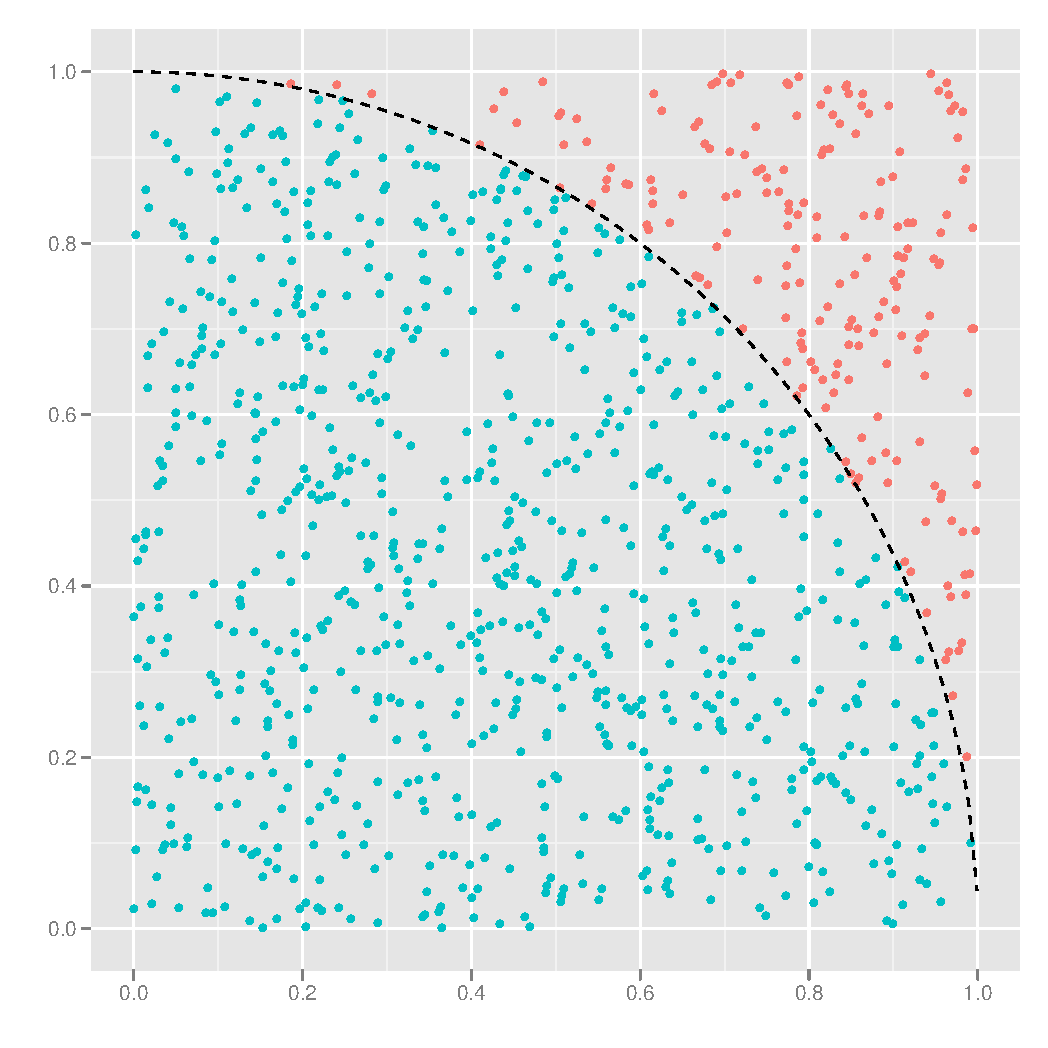
\includegraphics[scale=.25]{pics/pi} 
  \end{center}
  \end{block}
\end{frame}


\begin{frame}[fragile]
  \begin{block}{Example \showex :  Monte Carlo Simulation SPMD Algorithm}\pause
    \begin{enumerate}
     \item Let $n$ be big-ish; we'll take $n=50,000$.
     \item Generate an $n\times 2$ matrix $x$ of standard uniform observations.
     \item Count the number of rows satisfying $x^2 + y^2 \leq 1$
     \item Ask everyone else what their answer is; sum it all up.
     \item Take this new answer, multiply by 4 and divide by $n$
     \item If my rank is 0, print the result.
    \end{enumerate}
  \end{block}
\end{frame}


\begin{frame}[fragile,scale,shrink]
  \begin{exampleblock}{Example \showex :  Monte Carlo Simulation Code}\pause
\begin{lstlisting}[title=Serial Code]
N <- 50000
X <- matrix(runif(N * 2), ncol=2)
r <- sum(rowSums(X^2) <= 1)
PI <- 4*r/N
print(PI)
\end{lstlisting}

\begin{lstlisting}[title=Parallel Code]
library(pbdMPI, quiet = TRUE)
init()
comm.set.seed(diff=TRUE)

N.spmd <- 50000 / comm.size()
X.spmd <- matrix(runif(N.spmd * 2), ncol = 2)
r.spmd <- sum(rowSums(X.spmd^2) <= 1)
r <- allreduce(r.spmd)
PI <- 4*r/(N.spmd * comm.size())
comm.print(PI)

finalize()
\end{lstlisting}
  \end{exampleblock}
\end{frame}

\begin{frame}[fragile]
  \begin{block}{Note}\pause
    For the remainder, we will exclude loading, init, and finalize calls.
  \end{block}
\end{frame}










\subsection{pbdMPI Example: Sample Covariance}

\begin{frame}
  \begin{block}{Example \countex :  Sample Covariance}\pause
  \begin{align*}
    cov(x_{n\times p}) = \frac{1}{n-1}\sum_{i=1}^n\left(x_i-\mu_x\right)\left(x_i-\mu_x\right)^T
  \end{align*}
  \end{block}
\end{frame}


\begin{frame}
  \begin{block}{Example \showex :  Sample Covariance SPMD Algorithm}\pause
    \begin{enumerate}
     \item Determine the total number of rows $N$.
     \item Compute the vector of column means of the full matrix.
     \item Subtract each column's mean from that column's entries in each local matrix.
     \item Compute the crossproduct locally and reduce.
     \item Divide by $N-1$.
    \end{enumerate}
  \end{block}
\end{frame}


\begin{frame}[fragile,shrink]
  \begin{exampleblock}{Example \showex :  Sample Covariance Code}\pause
\begin{lstlisting}[title=Serial Code]
N <- nrow(X)
mu <- colSums(X) / N

X <- sweep(X, STATS=mu, MARGIN=2)
Cov.X <- crossprod(X.spmd) / (N-1)

print(Cov.X)
\end{lstlisting}
  
\begin{lstlisting}[title=Parallel Code]
N <- allreduce(nrow(X.spmd), op="sum")
mu <- allreduce(colSums(X.spmd) / N, op="sum")

X.spmd <- sweep(X.spmd, STATS=mu, MARGIN=2)
Cov.X <- allreduce(crossprod(X.spmd), op="sum") / (N-1)

comm.print(Cov.X)
\end{lstlisting}
  \end{exampleblock}
\end{frame}







\subsection{pbdMPI Example: Linear Regression}

\begin{frame}
  \begin{block}{Example \countex :  Linear Regression}\pause
      Find $\bbeta$ such that
      \begin{align*}
      \by = \bX\bbeta + \bepsilon
      \end{align*}

      When $\bX$ is full rank,
      \begin{align*}
      \hat{\bbeta} = (\bX^T\bX)^{-1}\bX^T\by \label{math:ols}
      \end{align*}
  \end{block}
\end{frame}


\begin{frame}
  \begin{block}{Example \showex :  Linear Regression SPMD Algorithm}\pause
    \begin{enumerate}
     \item Locally, compute $tx = x^T$
     \item Locally, compute $A = tx * x$. Query every other processor for this result and sum up all the results.
     \item Locally, compute $B = tx * y$.  Query every other processor for this result and sum up all the results.
     \item Locally, compute $A^{-1} * B$
    \end{enumerate}
  \end{block}
\end{frame}


\begin{frame}[fragile,shrink]
  \begin{exampleblock}{Example \showex :  Linear Regression Code}\pause
\begin{lstlisting}[title=Serial Code]
tX <- t(X)
A <- tX %*% X
B <- tX %*% y

ols <- solve(A) %*% B
\end{lstlisting}
  
\begin{lstlisting}[title=Parallel Code]
tX.spmd <- t(X.spmd)
A <- allreduce(tX.spmd %*% X.spmd, op = "sum")
B <- allreduce(tX.spmd %*% y.spmd, op = "sum")

ols <- solve(A) %*% B
\end{lstlisting}
  \end{exampleblock}
\end{frame}